\section{Resultados}
\begin{frame}
\frametitle{Anti-thickness geométrico}
Para $3 \leq n \leq 10$:
\[  At_g(K_n) = n - \left\lfloor\sqrt{2n + \frac{1}{4}} - \frac{1}{2} \right\rfloor \]
\end{frame}
\begin{frame}
\frametitle{Estado del arte}
Para $n \geq 3$:
\[  \frac{n-1}{2} \leq At_g(K_n) \leq n - \left\lfloor\sqrt{2n + \frac{1}{4}} - \frac{1}{2} \right\rfloor \]
Para encontrar alguna cota inferior es posible explotar alguna propiedad que se cumpla para todas las gráficas geométricas de $K_n$. Para encontrar una cota superior es posible ofrecer una descomposición de $K_n$ en thrackles.
\end{frame}
\begin{frame}
\frametitle{Estado del arte : cota inferior}
Erd\H{o}s \emph{et al.} probaron que cada gráfica geométrica con $n$ vértices en la cual no existen dos aristas disjuntas tiene a lo sumo $n$ aristas. 
\\[10pt]
Esto quiere decir que un thrackle máximo tiene a lo sumo $n$ aristas.
\end{frame}
\begin{frame}
\frametitle{Estado del arte : cota inferior}
En el trabajo de Wood \& Dujmovic se menciona que para $n \geq 3$:
\[  \frac{n-1}{2} \leq At_g(K_n).\] 
\pause

Esta cota inferior es la más sencilla, se basa en la noción del número máximo de aristas en un thrackle máximo. 
\\[5pt]
Si la gráfica completa tiene $\binom{n}{2} = \frac{n(n-1)}{2}$ aristas, ¿cuántos thrackles máximos son necesarios para \emph{cubrir} todas las aristas? Si suponemos que $k$ thrackles máximos son necesarios la siguiente desigualdad nos otorga el resultado si resolvemos para $k$: \[ k\cdot n \geq \frac{n(n-1)}{2} \pause \Rightarrow k = \frac{n-1}{2}\]
\end{frame}

\begin{frame}
\frametitle{Estado del arte : cota superior}
Fabila-Monroy \emph{et al.} encuentran el anti-thickness exacto del dibujo convexo de $K_n$. Ellos se enfocan en el número cromático de $D(S)$, para la cota inferior establecen el número mínimo de colores necesarios en una coloración propia de $D(S)$ y para la cota superior dan una coloración propia para cualquier $n$, con $n>3$.
\pause 
\\[10pt]
Ellos establecen que $\chi(D(S)) = n - \left\lfloor\sqrt{2n + \frac{1}{4}} - \frac{1}{2} \right\rfloor, $ cuando $S$ está en posición convexa.
\pause
\\[10pt]
Como la posición convexa es un dibujo de $K_n$ tenemos: \[At_g(K_n) \leq n - \left\lfloor\sqrt{2n + \frac{1}{4}} - \frac{1}{2} \right\rfloor. \]
\end{frame}
\begin{frame}
\frametitle{Estado del arte : thrackles máximos en posición convexa}
Un resultado del trabajo de Fabila-Monroy \emph{et al.} es que prueban que dos thrackles máximos en posición convexa siempre comparten al menos una arista. Esto significa que, en posición convexa, una descomposición por $k$ thrackles máximos cubre a lo sumo $kn - \binom{k}{2}$ aristas. Para obtener el valor más pequeño de $k$ podemos resolver, para $k$, la siguiente desigualdad :
\[
  kn - \binom{k}{2} \geq \binom{n}{2}.
\]
Usando la ecuación cuadrática encontramos que $k = n - \left\lfloor\sqrt{2n + \frac{1}{4}} - \frac{1}{2} \right\rfloor.$
\end{frame}
\begin{frame}
\begin{figure}
	\centering
	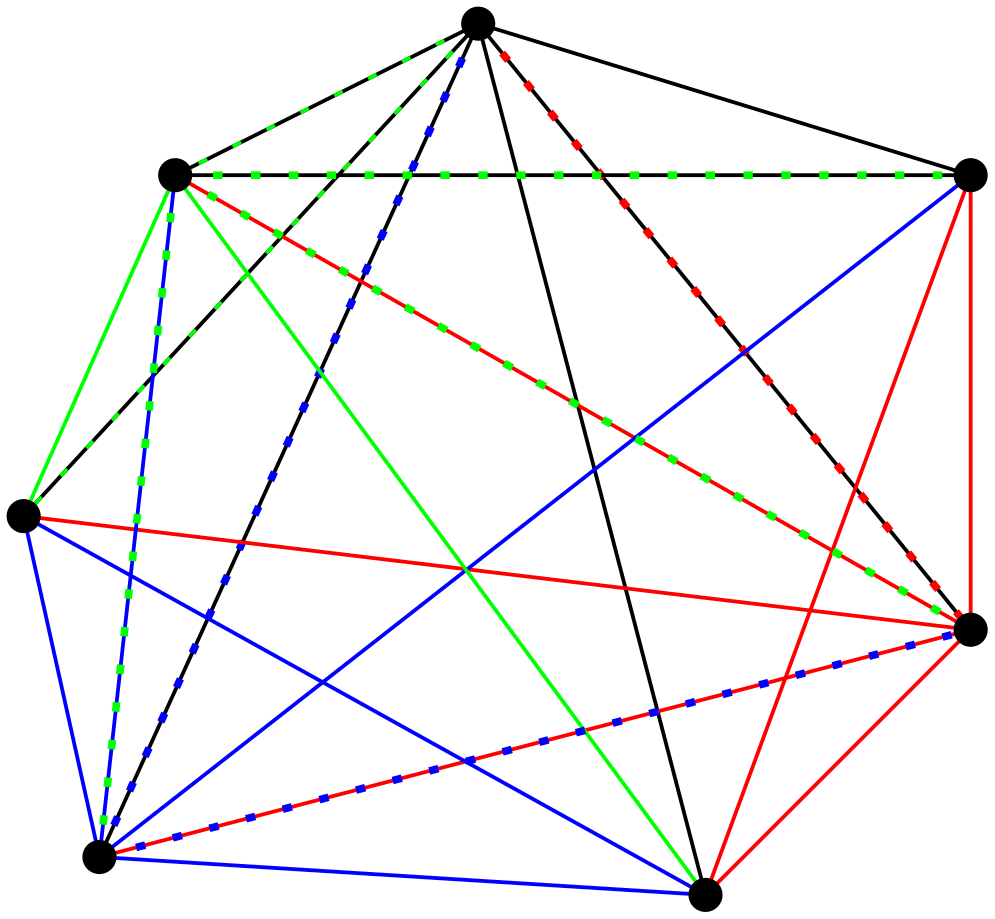
\includegraphics[width=0.75\linewidth]{images/thrackles_maximos}
\end{figure}
\end{frame}

\begin{frame}
\frametitle{Estado del arte : thrackles máximos en posición general}
\pause
\begin{itemize}
	\item En posición general es muy dificil dibujar thrackles máximos que sean disjuntos.
	\item La intuición nos dice que el resultado anterior es válido para posición general.
	\item ¿Cómo probamos \emph{todos} las gráficas geométricas de $K_n$?
\end{itemize}
\end{frame}

\begin{frame}
\frametitle{Tipo de orden}
\end{frame}

\begin{frame}
\frametitle{Estado del arte : construyendo la nueva cota inferior}
\end{frame}